 \documentclass{article}

% cursor parking lot please place 
% your cursor here when you go away
% so other's can work :) 
% -------------------------
% |     |     |     |     |
% |     |     |     |     |
% -------------------------

% libraries
\usepackage{amsmath, amssymb, hyperref, fullpage, enumitem, graphicx, subcaption, float, braket} 

% ignore these ... 
\setlength{\parindent}{0pt}
\setlength{\parskip}{\medskipamount}
\setcounter{secnumdepth}{-2}

\begin{document}

These notes follow \href{https://sigma-journal.com/2010/039/sigma10-039.pdf}{Wehefritz-Kaufmann}, and were produced collaboratively by Esha Sury and Dhruv Upreti.

\section{Totally Asymmetric Diffusion on a Ring}

Note that the two species asymmetric diffusion model consists of two species of particles, $A$ and $B$, diffusing asymmetrically in one dimension. The following processes take place:

\[
\begin{array}{lll}
A + 0 \to 0 + A & \text{with rate } \Gamma_R, 
& 0 + A \to A + 0 \quad \text{with rate } \Gamma_L, \\[4pt]
B + 0 \to 0 + B & \text{with rate } \Gamma_R, 
& 0 + B \to B + 0 \quad \text{with rate } \Gamma_L, \\[4pt]
A + B \to B + A & \text{with rate } \Gamma_R, 
& B + A \to A + B \quad \text{with rate } \Gamma_L.
\end{array}
\] 

In the totally asymmetric case, $\Gamma_L =0$ meaning that particles $A$ don't diffuse to the left. The image in the Figure 1(a) below shows the asymmetric diffusion with periodic boundary conditions (on the ring $\mathbb{Z}/L\mathbb{Z}$). Note from the asymmetric model both $A$ and $B$ can move into vacancies, but when $A$ and $B$ meet, $A$ has priority since $A + B \to B + A$ and $B + A \not\to A + B$. Therefore $A$ are called a \textbf{first-class} particles and $B$ are called a \textbf{second-class} particles.  

\begin{figure}[H]
    \centering
    \begin{subfigure}[b]{0.4\linewidth}
        \centering
        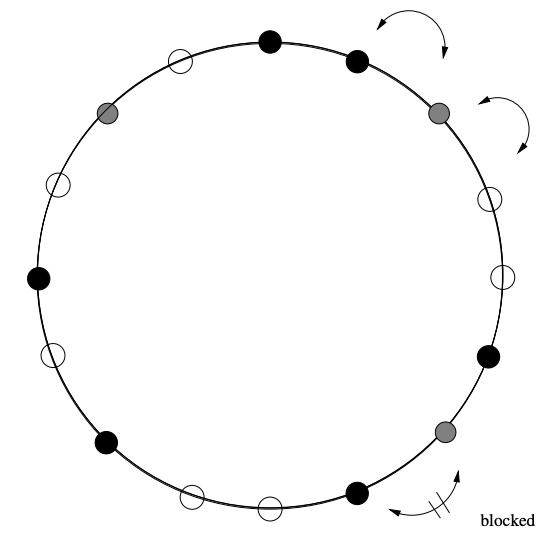
\includegraphics[width=\linewidth]{figures/asym_diffusion_on_ring.png}
        \caption{Black dots correspond to $A$, grey dots to $B$ and open dots to $0$ or vacancies.}
    \end{subfigure} \hfill
    \begin{subfigure}[b]{0.4\linewidth}
        \centering
    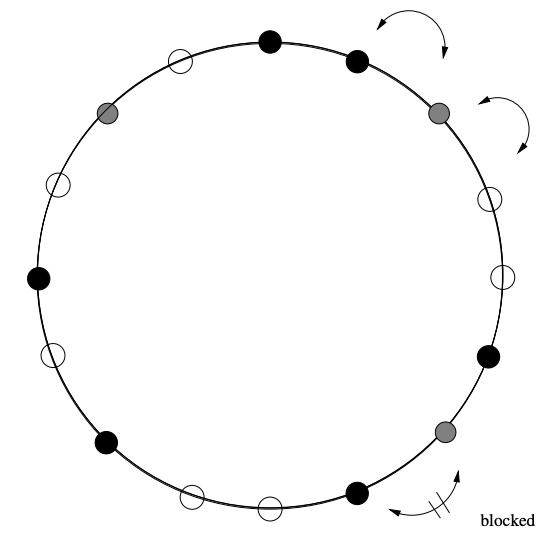
\includegraphics[width=\linewidth]{figures/asym_diffusion_on_ring.png}
        \caption{}
    \end{subfigure}
    \caption{}
\end{figure}

\subsection{Master Equation and Markov Generator}

In math and physics \href{https://en.wikipedia.org/wiki/Master_equation}{master equations} are used to describe the time evolution of a system that can be modeled as being in a probabilistic combination of states at any given time. In a nutshell in a master equation it is said that

\[\frac{d}{dt}p_t(\eta) = \text{prob. system in configuration $\eta$ at time $t$} = \text{prob. flowing into $\eta$} - \text{prob. flowing out of $\eta$}.\]

Take an example of a two state system where the probability of being in each state is $p_1(t)$ for state $1$ and $p_2(t)$ for state $2$ and the rates of transition are given as 

\[1 \to 2 \text{ with rate: $r$}, \quad 2\to1 \text{ with rate: $s$}.\]

Note that then the master equation can be written as,

\[\frac{dp_1}{dt} = sp_2 -rp_1, \quad \frac{dp_2}{dt} = rp_1 - sp_2 \Rightarrow \frac{d}{dt}\begin{pmatrix}p_1 \\ p_2 \end{pmatrix} = \begin{pmatrix} -r & s \\ r & -s \end{pmatrix} \begin{pmatrix} p_1 \\ p_2 \end{pmatrix}.\]

The matrix is known as the \textbf{Markov generator} and the off diagonal elements are the transition rates while the diagonal entries are the negative escape rates (to make sure the total probability is conserved so that $p_1(t) + p_2(t) = 1$). For a system with many states $\eta_1, \eta_2, \dots$ we say that $W_{\eta,\eta'}$ is the jump rate from configuration $\eta$ to $\eta'$. The master equation then becomes,

\[\frac{d}{dt}p_t(\eta) = \sum_{\eta\neq \eta'}\left[W_{\eta,\eta'} p_t(\eta) - W_{\eta',\eta}p_t(\eta)\right].\]

Written in matrix form this is,

\[\frac{d}{dt}\ket{P(t)} = M\ket{P(t)}.\]

Where $\ket{P(t)}$ is the vector of all probabilities. Note that this is exactally the \href{https://en.wikipedia.org/wiki/Schr%C3%B6dinger_equation#Time-dependent_equation}{time dependent Schrodinger} equation in imaginary time, where the negative of the Markov generator, $-M$, represents the Hamiltonian. The solution is known to be,

\[\ket{P(t)} = e^{Mt}\ket{P(0)} = e^{-Ht}\ket{P(0)}.\]

Notice how this differs from the real time solution of the Schrodinger equation where $\ket{\psi(t)} = e^{-iHt}\ket{\psi(0)}$. Fundamentally the difference is that the factor $e^{-iHt}$ oscillates while $e^{-Ht}$ decays. Therefore in a stochastic process the eigenvalues of $H$ are not physical energies, they are decay or \textbf{relaxation times}. 

For the diffusion model we say that $\eta$ is the arrangement of $A,B$ and $0$ around the ring. Since the allowed moves are just the nearest neighbor swaps the configurations connected to $\eta$ are just configurations obtained by swapping neighboring sites so, 

\[\frac{d}{dt} p_t(\eta) = \sum_j \left[c(j,j+1,\eta^{j,j+1})p_t(\eta^{j,j+1}) - c(j,j+1,\eta)p_t(\eta)\right].\]

Here $\eta^{j,j+1}$ is the configuration obtained by changing the sites $j$ and $j+1$ from $\eta$. In the formula above the term,

\[-c(j,j+1,\eta)p_t(\eta)\]

represents the "loss" and states if the system is in configuration $\eta$ then the pair at sites $j$ and $j+1$ may exchange with a rate $-c(j,j+1,\eta)$. The term,

\[c(j,j+1,\eta^{j,j+1})p_t(\eta^{j,j+1})\]

is the "gain" term and states if the system is in configuration $\eta^{j,j+1}$ then exchanging the cites will produce the configuration $\eta$. 

\subsection{Asymmetric Diffusion Hamiltonian}

In order to write the full Hamiltonian, we realize that the site can be in one of three states which are represented as basis vectors of $\mathbb{C}^3$ with the following labeling: 

\[A = \begin{pmatrix}1 \\ 0 \\ 0\end{pmatrix}\sim 1, \quad B = \begin{pmatrix}0 \\ 1 \\ 0\end{pmatrix}\sim 2,\quad 0 = \begin{pmatrix}0 \\ 0 \\ 1\end{pmatrix}\sim 3\]

The full configuration on a ring of length $L$ then becomes the tensor product: $\left(\mathbb{C}^3\right)^{\otimes L}$. Now, recall that the asymmetric model's moves from above. Using the labels,

\[1\sim A, \quad 2 \sim B, \quad 3 \sim 0,\]

the right and left moves are exactally,

\begin{align*}
\ket{\alpha,\beta} \rightarrow& \ket{\beta, \alpha}, \quad \text{when $\alpha < \beta$ with exchange rate $\Gamma_R$} \\
\ket{\alpha,\beta}\rightarrow& \ket{\beta,\alpha}, \quad \text{when $\beta< \alpha$ with exchange rate $\Gamma_L$.}
\end{align*}

In order to define these exchanges the $3\times3$ matrix operator $E^{\alpha\beta}$ is used that turns basis state $\beta$ in to state $\alpha$, 

\[E^{\alpha\beta}\ket{\gamma} = \delta_{\beta\gamma}\ket{\alpha}.\]

On the on the site $j$ the exchange tensor is written as $E_{j}^{\alpha\beta} = I\otimes\cdots\otimes E^{\alpha\beta} \otimes\cdots\otimes I$. Therefore we see that the product $E^{\alpha\beta}_j E^{\beta\alpha}_{j+1}$ on a local pair $\ket{\beta,\alpha}$ is,

\[E_{j}^{\alpha\beta} E_{j+1}^{\beta\alpha} \ket{\beta,\alpha} = \ket{\alpha,\beta}.\]

Note that the master equation splits into two types of terms, the off diagonal parts which represent the transition terms and the diagonal part which represent the escape rate terms. For the Markov generator the off diagonal entries are positive transition rates while the diagonal entries are negative escape rates. For the Hamiltonian the opposite sign convention is used, since $H=-M$, so the off diagonal entries are negative transition rates and the diagonal entries are positive escape rates. Understanding this sign convention is key to the next part. 

Recall the off diagonal transitions are exchanges of neighboring states so for $\alpha<\beta$ the exchange rate is $\Gamma_R$, and for $\alpha>\beta$ the exchange rate is $\Gamma_L$. If we define $D=\sqrt{\Gamma_R\Gamma_L}$, and $q=\sqrt{\Gamma_R/\Gamma_L}$ such that $Dq = \Gamma_R$ and $Dq^{-1}=\Gamma_L$ then the off diagonal term becomes,

\[-Dq\sum_{\alpha<\beta} E^{\alpha\beta}_j E^{\beta\alpha}_{j+1} - Dq^{-1}\sum_{\alpha>\beta} E^{\alpha\beta}_j E^{\beta\alpha}_{j+1}.\]

The diagonal escape term follows similarly as,

\[Dq\sum_{\alpha<\beta} E^{\alpha\alpha}_{j} E^{\beta\beta}_{j+1} + Dq^{-1} \sum_{\alpha>\beta} E^{\alpha\alpha}_{j} E^{\beta\beta}_{j+1}.\]

The total Hamiltonian becomes,

\begin{align*} 
    H &= D\sum_{j=1}^L\left[-q\sum_{\alpha<\beta} E^{\alpha\beta}_j E^{\beta\alpha}_{j+1} - q^{-1}\sum_{\alpha>\beta} E^{\alpha\beta}_j E^{\beta\alpha}_{j+1} + q\sum_{\alpha<\beta} E^{\alpha\alpha}_{j} E^{\beta\beta}_{j+1} + q^{-1} \sum_{\alpha>\beta} E^{\alpha\alpha}_{j} E^{\beta\beta}_{j+1}\right] \\ 
    &= D \sum_{j=1}^{L} \left[ \frac{q+q^{-1}}{2} - q \sum_{\alpha<\beta} E_j^{\alpha\beta} E_{j+1}^{\beta\alpha} - q^{-1} \sum_{\alpha>\beta} E_j^{\alpha\beta} E_{j+1}^{\beta\alpha} \right. \\ 
    &\qquad\qquad\qquad\qquad\qquad \left. -\frac{q+q^{-1}}{2} \sum_{\alpha=1}^{3} E_j^{\alpha\alpha} E_{j+1}^{\alpha\alpha} - \frac{q-q^{-1}}{2} \sum_{\alpha\ne\beta} \operatorname{sign}(\alpha-\beta) E_j^{\alpha\alpha} E_{j+1}^{\beta\beta} \right]. 
\end{align*}

The second form, written in the paper, is algebraically equivalent. Where realize that $E^{\alpha\alpha}_j$ represents the projector onto the state $\alpha$ at $j$,

\[E^{\alpha\alpha}\ket{\gamma} = \delta_{\alpha\gamma}\ket{\alpha}, \quad E^{\alpha\alpha}_j E^{\beta\beta}_{j+1} \ket{\gamma, \nu} = \delta_{\alpha\gamma}\delta_{\beta\nu}\ket{\alpha,\beta}.\]

This Hamiltonian is integrable and the eigenvalues can be found by applying the \hyperref[sec:bethe-ansatz-on-asym-hamiltonian]{Bethe ansatz}.

\subsection{Dynamical Critical Exponent}

The dynamical critical exponent describes a relation between the relaxation time towards equilibrium $\tau$ (or temporal correlation length) of a system and the spatial correlation length $\xi$. Note that 

\subsection{Bethe Ansatz on Asymmetric Diffusion Hamiltonian}
\label{sec:bethe-ansatz-on-asym-hamiltonian}

\subsection{Analytical Solution to Bethe Ansatz}

\section{Bethe Ansatz}
\label{sec:bethe-ansatz}



\end{document}